\documentclass[t]{beamer}\usepackage[]{graphicx}\usepackage[table]{xcolor}
% maxwidth is the original width if it is less than linewidth
% otherwise use linewidth (to make sure the graphics do not exceed the margin)
\makeatletter
\def\maxwidth{ %
  \ifdim\Gin@nat@width>\linewidth
    \linewidth
  \else
    \Gin@nat@width
  \fi
}
\makeatother

\definecolor{fgcolor}{rgb}{0.345, 0.345, 0.345}
\newcommand{\hlnum}[1]{\textcolor[rgb]{0.686,0.059,0.569}{#1}}%
\newcommand{\hlsng}[1]{\textcolor[rgb]{0.192,0.494,0.8}{#1}}%
\newcommand{\hlcom}[1]{\textcolor[rgb]{0.678,0.584,0.686}{\textit{#1}}}%
\newcommand{\hlopt}[1]{\textcolor[rgb]{0,0,0}{#1}}%
\newcommand{\hldef}[1]{\textcolor[rgb]{0.345,0.345,0.345}{#1}}%
\newcommand{\hlkwa}[1]{\textcolor[rgb]{0.161,0.373,0.58}{\textbf{#1}}}%
\newcommand{\hlkwb}[1]{\textcolor[rgb]{0.69,0.353,0.396}{#1}}%
\newcommand{\hlkwc}[1]{\textcolor[rgb]{0.333,0.667,0.333}{#1}}%
\newcommand{\hlkwd}[1]{\textcolor[rgb]{0.737,0.353,0.396}{\textbf{#1}}}%
\let\hlipl\hlkwb

\usepackage{framed}
\makeatletter
\newenvironment{kframe}{%
 \def\at@end@of@kframe{}%
 \ifinner\ifhmode%
  \def\at@end@of@kframe{\end{minipage}}%
  \begin{minipage}{\columnwidth}%
 \fi\fi%
 \def\FrameCommand##1{\hskip\@totalleftmargin \hskip-\fboxsep
 \colorbox{shadecolor}{##1}\hskip-\fboxsep
     % There is no \\@totalrightmargin, so:
     \hskip-\linewidth \hskip-\@totalleftmargin \hskip\columnwidth}%
 \MakeFramed {\advance\hsize-\width
   \@totalleftmargin\z@ \linewidth\hsize
   \@setminipage}}%
 {\par\unskip\endMakeFramed%
 \at@end@of@kframe}
\makeatother

\definecolor{shadecolor}{rgb}{.97, .97, .97}
\definecolor{messagecolor}{rgb}{0, 0, 0}
\definecolor{warningcolor}{rgb}{1, 0, 1}
\definecolor{errorcolor}{rgb}{1, 0, 0}
\newenvironment{knitrout}{}{} % an empty environment to be redefined in TeX

\usepackage{alltt}
\usepackage{graphicx} % Required for inserting images
\usepackage{booktabs} % For better tables
\usepackage[absolute,overlay]{textpos}
\usepackage{multirow}
\usepackage[table]{xcolor} % for color backgrounds
\usepackage{array}
\setbeamertemplate{itemize item}[circle]
\setbeamertemplate{itemize subitem}[square]
\setbeamertemplate{section in toc}[ball unnumbered]
\setbeamertemplate{subsection in toc}[circle]
\usepackage{amsmath,amsthm}
\usepackage{Sweave} % Required for Rnw files

\usetheme{Dresden}
\setbeamertemplate{headline}{
  \leavevmode%
  \hbox{%
    \begin{beamercolorbox}[wd=\paperwidth,ht=2.5ex,dp=1ex,left]{section in head/foot}
      \hspace*{1em}\insertsection
    \end{beamercolorbox}%
  }
}

\addtobeamertemplate{frametitle}{}{%
    \begin{textblock*}{1cm}(1.11\textwidth,1.105\textheight)
        \color{white}\tiny\insertframenumber{} / \inserttotalframenumber
    \end{textblock*}
}


% --- Presentation information ---
\title{Replication: Factor Momentum}
\subtitle{Based on Arnott, Clements, Kalesnik, Linnainmaa (2021)}
\author{Your Name/Group Name} % <<<--- CHANGE THIS
\institute[WU PMP Vienna]{Portfolio Management Program \\ WU Vienna} % <<<--- Adjust if needed
\date{\today} % Or set a specific date
\IfFileExists{upquote.sty}{\usepackage{upquote}}{}
\begin{document}

% --- Title Frame (Using a generic background, replace Picture 3.png if needed) ---
{
% \usebackgroundtemplate{\includegraphics[width=\paperwidth,height=\paperheight]{Picture 3.png}} % Uncomment if you have the image
\begin{frame}[plain]
    \titlepage % Use standard title page layout
\end{frame}
}

% --- Table of Contents ---
\begin{frame}{Table of Contents}
    \tableofcontents
\end{frame}

% --- Setup Chunk (Hidden) ---


% --- Section: Replication Results ---
\section{Replication Results}

\begin{frame}{Outline}
    \tableofcontents[currentsection,hideallsubsections]
\end{frame}

\begin{frame}{Factor vs. Industry Momentum Performance}
\textbf{Methodology:}
% Corrected itemize environment
\begin{itemize}
    \item Implement 1-month formation, 1-month holding momentum strategy.
    \item Applied to 17 Fama-French industry portfolios and selected JKP factors.
    \item Long assets above median prior return, short assets below median.
    \item Equal-weighted within long/short legs, rebalanced monthly.
    \item Sample: July 1963 - December 2024 (USA Data).
\end{itemize}

\vspace{0.5cm} % Add some vertical space

\end{frame}

\begin{frame}

\begin{knitrout}
\definecolor{shadecolor}{rgb}{0.969, 0.969, 0.969}\color{fgcolor}\begin{figure}

{\centering 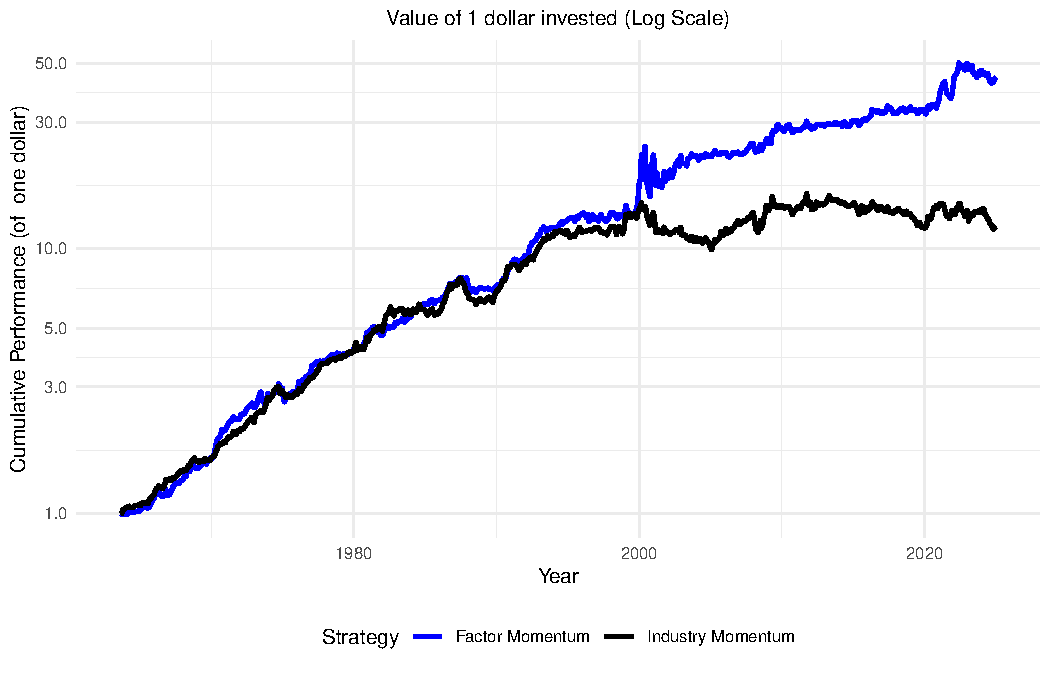
\includegraphics[width=\maxwidth]{figure/cum_ret_plot-1} 

}

\caption[Cumulative Performance (Log Scale), July 1963 - Dec 2020]{Cumulative Performance (Log Scale), July 1963 - Dec 2020}\label{fig:cum_ret_plot}
\end{figure}

\end{knitrout}

\end{frame}

\begin{frame}{Factor Correlation Heatmap}
\textbf{Analysis:}
\begin{itemize}
    \item Correlation calculated among the selected JKP factors used in the factor momentum strategy.
    \item Helps understand the relationships between the factors being timed.
\end{itemize}

\vspace{0.5cm} % Add some vertical space
\end{frame}


\begin{frame}
\begin{knitrout}
\definecolor{shadecolor}{rgb}{0.969, 0.969, 0.969}\color{fgcolor}\begin{figure}

{\centering 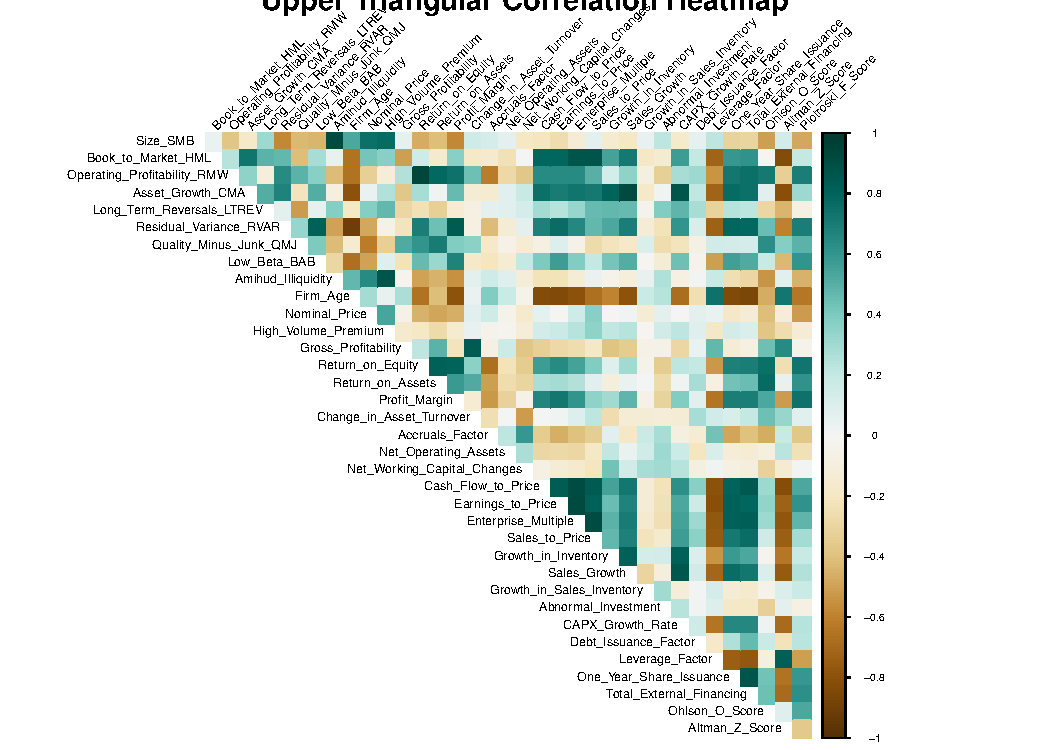
\includegraphics[width=\maxwidth]{figure/corr_heatmap1-1} 

}

\caption[Upper Triangular Correlation Heatmap of Selected JKP Factors]{Upper Triangular Correlation Heatmap of Selected JKP Factors}\label{fig:corr_heatmap1}
\end{figure}

\end{knitrout}

\end{frame}


\begin{frame}
\begin{knitrout}
\definecolor{shadecolor}{rgb}{0.969, 0.969, 0.969}\color{fgcolor}\begin{figure}

{\centering 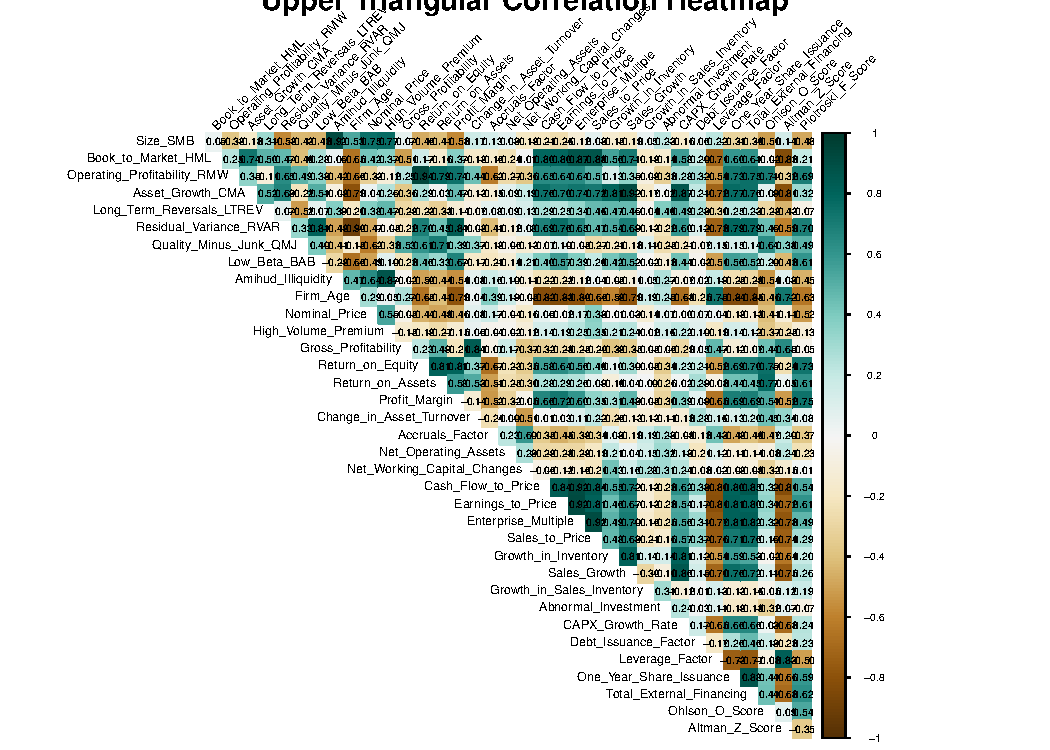
\includegraphics[width=\maxwidth]{figure/corr_heatmap-1} 

}

\caption[Upper Triangular Correlation Heatmap of Selected JKP Factors]{Upper Triangular Correlation Heatmap of Selected JKP Factors}\label{fig:corr_heatmap}
\end{figure}

\end{knitrout}

\end{frame}

\begin{frame}{Key Findings \& Conclusion}
% Corrected itemize environment
\begin{itemize}
    \item \textbf{Replication Findings:}
        \begin{itemize}
            \item Both industry and factor momentum strategies generated positive returns over the 1963-2020 period.
            \item The cumulative performance plot visually suggests factor momentum was significantly stronger and more persistent, especially in later years, mirroring Figure 1 in Arnott et al. (2021).
            \item Factor correlations vary, indicating diversification benefits within the factor universe itself.
        \end{itemize}
    \item \textbf{Connection to Arnott et al. (2021):}
        \begin{itemize}
            \item The paper argues that factor momentum \textit{subsumes} industry momentum. While this R code doesn't perform the formal spanning regressions from the paper (Table 4), the performance difference is suggestive.
            \item Arnott et al. show that momentum concentrates in high-eigenvalue principal component factors derived from industry-neutral factors. Our analysis uses the raw JKP factors directly.
        \end{itemize}
     \item \textbf{Conclusion:} The results support the presence of short-term momentum in both industries and factors. The superior performance of the factor momentum strategy aligns with the central thesis of Arnott et al. (2021) that factor dynamics are the primary driver. % Removed emoji
\end{itemize}

\end{frame}

\end{document}
